
\chapter{Introdução}

\label{CapIntro}

% Resumo opcional. Comentar se não usar.
% \resumodocapitulo{Resumo opcional}

\par O interesse humano em criar artefatos para facilitar seu próprio trabalho ou realizar uma tarefa sem interferência remonta os tempos mais antigos. No Egito Ptolomaico, Ctesíbio (285-222 AC) descreveu um relógio d`água com a presença de um sistema de engrenagens, um indicador e o primeiro sistema de retroalimentação registrado. Por volta de 1495, Leonardo da Vinci, concebeu o projeto de um autômato mecânico de um guerreiro em armadura medieval que podia ficar em pé, sentar-se, levantar o visor e mover os braços. \cite{guarnieri2010} 
\par O estudo da união de sistemas eletromecânicos e inteligência teve começo há pelo menos 70 anos. A \textit{cibernética}, área inaugurada por Norbert Wiener na década de 1950, descreve o estudo científico de controle e comunicação no animal e na máquina. Wiener começou, então, a desenvolver sistemas que replicassem comportamentos animais.\cite{wiener1950} Somado a isso, a teoria da informação de Claude Shannon e a teoria de computação de Alan Turing abriram espaço para pesquisas que iriam desenvolver Inteligências Artificiais (IA). \cite{pamela2004} 

\section{Robótica}
\par A robótica se apoia em conhecimentos de vários campos para criar uma das áreas de estudos mais amplas da ciência. Desde a metade do século XX, a robótica vêm reunindo noções dessas áreas, e pouco a pouco as tornando partes essenciais de si: sistemas mecânicos, eletromecânicos, teoria de controle, IA e outras. As aplicações existentes são inúmeras e se renovam a todo momento. Dentre as principais, é possível citar sistemas de manufatura, robótica médica e robótica agricultural. \cite{handbook2007} 
\par Sistemas robóticos construídos para automatizar tarefas repetitivas são interessantes. Entretanto, o avanço das indústrias e aumento da complexidade das tarefas a serem realizadas criou um ambiente catalisador para o desenvolvimento de processos de tomada de decisão autonomamente. 
\par É importante notar a complexidade do problema de se desenvolver a tomada de decisão de um sistema autônomo. Tal sistema precisa mapear seu ambiente por meio de sensores, extrair um significado do seu estado atual, usá-lo para decidir uma ação e determinar se tal ação foi a melhor a ser tomada. Sensores, porém, são imprecisos e limitados fisicamente. A representação dos estados, frequentemente, não é completamente conhecida. E o processo de mapeamento de estado para ação não é trivial.
\par Neste contexto surgiu a área de estudo conhecida como \textit{aprendizagem por reforço}, que formaliza os elementos citados anteriormente para prover uma base de como agentes devem tomar ações para cumprir um objetivo pré-definido. \cite{sutton2018reinforcement}


\section{Aprendizagem por Reforço}

\section{Futebol de Robôs}
% TODO: detalhar histórico de futebol de robôs e falar de outras categorias de competição existentes

\subsection{RoboCup Soccer Simulation 2D}
\par A ideia de robôs jogando futebol foi proposta pela primeira vez em 1992 por Alan Mackworth\cite{mackworth1993seeing}.
Desde então a comunidade científica tem criado iniciativas buscando por soluções que tornem isso realidade.
Uma delas é a \textit{Robot World Cup Initiative}, abreviada como \textit{RoboCup}, que teve sua primeira edição em 1997 com mais de 40 equipes distribuídas entre as diversas categorias do evento.
\par O objetivo da iniciativa, definido pela \textit{RoboCup Federation}, é que por volta da metade do século XXI, um time de robôs humanóides autônomos vençam uma partida contra os campeões da Copa do Mundo mais recente. Mesmo que o objetivo pareça ambicioso, ele guia as pesquisas e motiva o avanço no campo.
Atualmente, a RoboCup conta com mais de 10 categorias, entre elas a \textit{RoboCup Soccer Simulation 2D}, abreviada RCSS, objeto de estudo deste projeto.
\par A categoria apresenta, também, grande relevância no cenário brasileiro.
Desde 2005, a RCSS está presente na maior competição de robótica da América Latina, a \textit{Latin American Robotics Competition}, LARC.
\par Nessa categoria, duas equipes de 11 jogadores autônomos e independentes jogam futebol em um ambiente virtual bidimensional.
Um servidor é responsável por esse ambiente e possui informação absoluta sobre o estado do jogo e suas regras.
Os jogadores, por sua vez, recebem dele informação incompleta e ruidosa de seus sensores virtuais, podendo executar comandos a fim de atuar sobre o estado do jogo.

\section{Caracterização do Problema}
% TODO: escrever sobre o problema de fazerr gols com aprondizagem por reforço

\subsection{Servidor da partida}
\par Um servidor que executa a partida é disponibilizado pelos organizadores da competição e este pode ser utilizado, também, para desenvolvimento. O servidor, portanto, apresenta, internamente, algumas das regras da partida bem como um juiz autônomo que age para determinar gols, faltas e demais situações de uma partida de futebol. Caso necessário, um juiz humano poderá intervir em situações não contempladas pelas regras do servidor.
\par O servidor simula todos os movimentos e ações dos jogadores e da bola. Clientes externos se conectam ao servidor e cada cliente controla um único jogador. A comunição entre o cliente e o servidor é feita a partir do protocolo UDP por meio de mensagens com sintaxe específica e definida pelo servidor.
\par De forma a permitir o acompanhamento visual da partida, um monitor também é disponibilizado, porém não é necessário para que uma partida ocorra com sucesso.
\par O servidor, ainda, possui o modo \textit{trainer} para utilização durante treinamentos de algoritmos de inteligência computacional. Este modo permite a conexão de um cliente do tipo treinador que tem acesso absoluto às informações da partida e pode mudar modos de jogo e ainda mover arbitrariamente jogadores e bola. Adicionalmente, é possível acelerar os ciclos da partida permitindo o treinamento em tempo hábil.

\begin{figure}[h]
	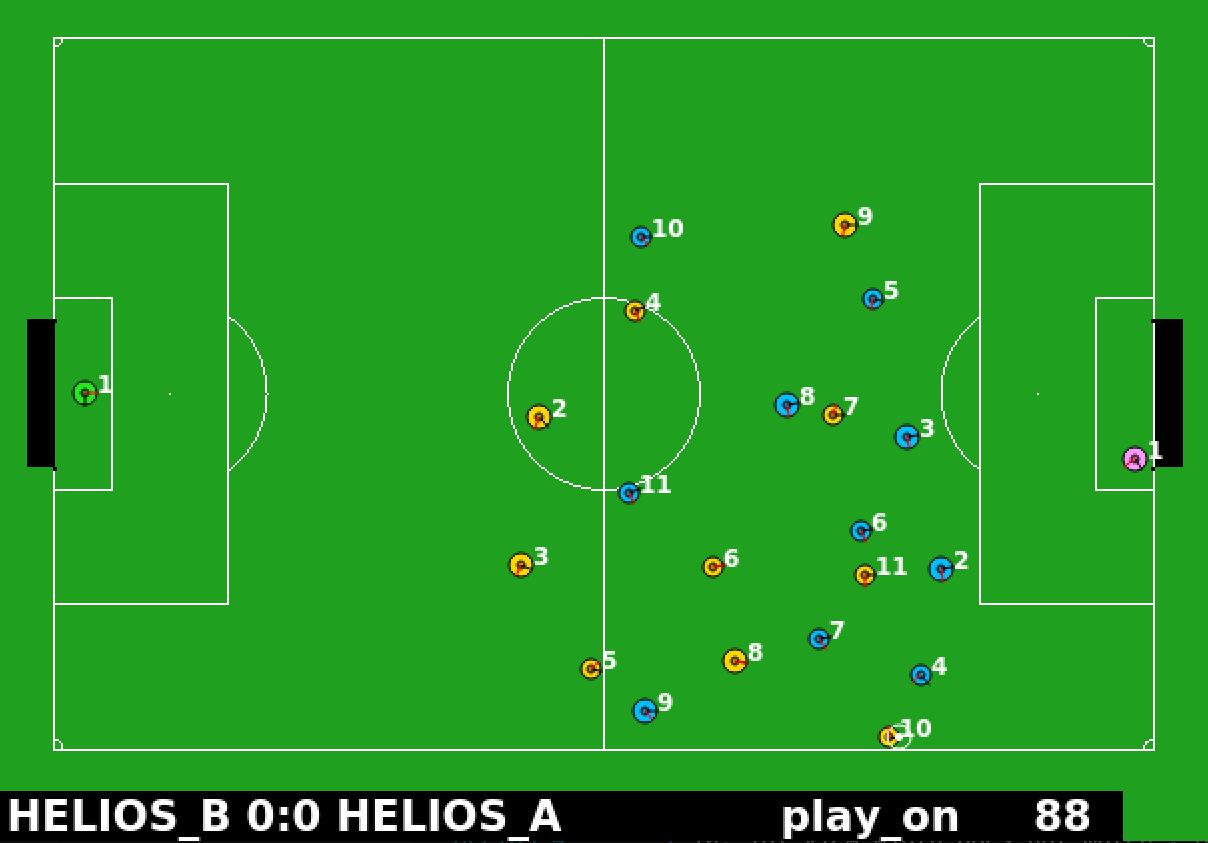
\includegraphics[width=0.7\linewidth]{figs/server.png}
	\centering
	\caption{Visualização de uma partida em andamento}
	\label{fig:rcssserver}
\end{figure}

\subsection{Cliente}
\par Os jogadores são controlados por clientes externos conectados ao servidor. Como já foi dito, um cliente corresponde a um único jogador e os clientes só podem ser comunicar com mensagens mandadas através do servidor da partida.
\par O cliente pode ser desenvolvido em qualquer linguagem desde que se comunique com o servidor pelo protocolo UDP e utilize a sintaxe de mensagens reconhecida pelo sistema. Há várias escolhas disponíveis para a construção do cliente, sendo decisão de cada equipe competidora como fazê-lo.

\begin{figure}[H]
	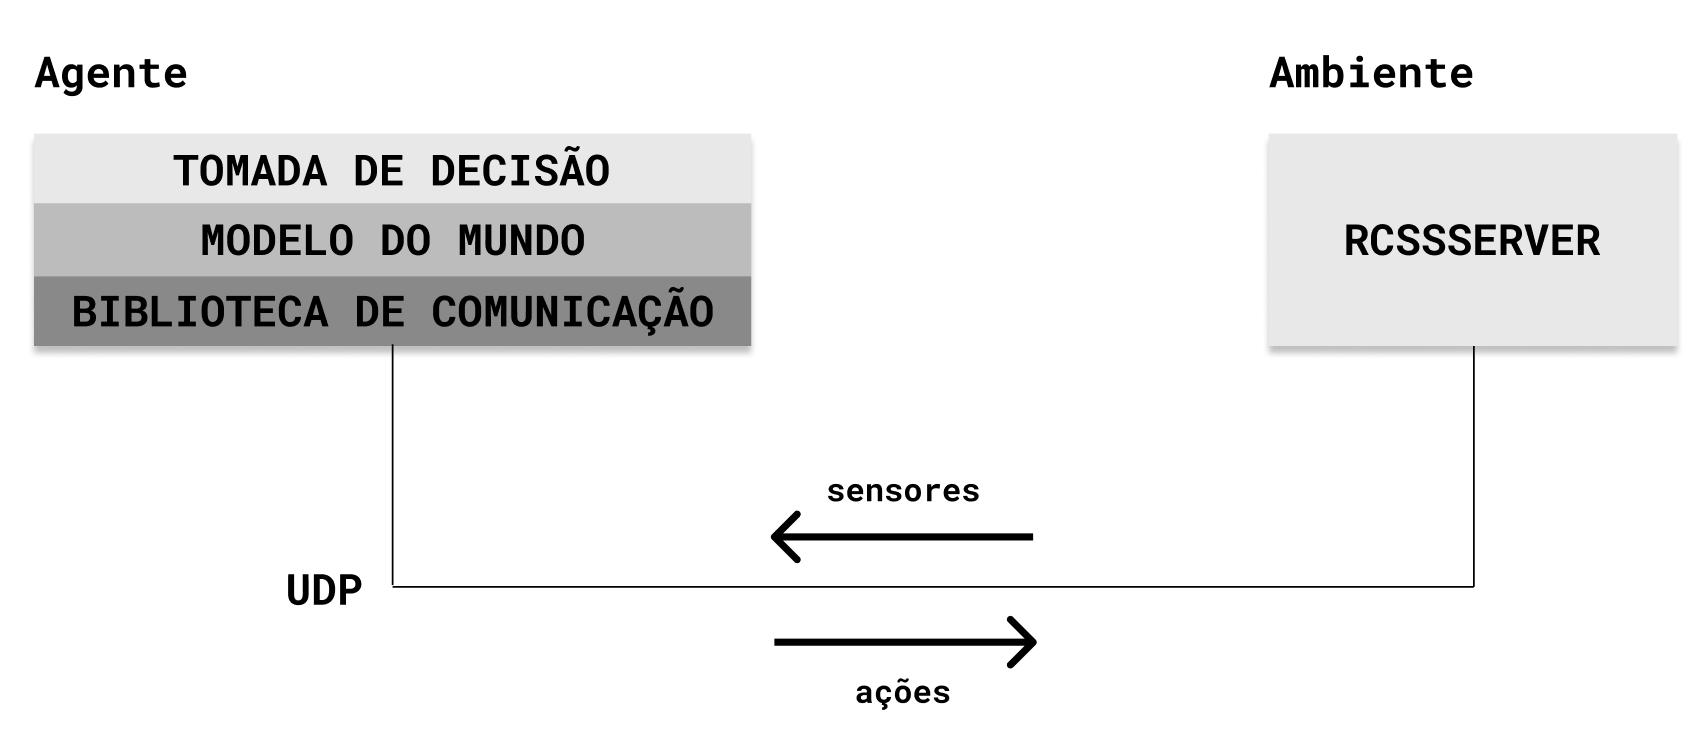
\includegraphics[width=0.9\linewidth]{figs/system.png}
	\centering
	\caption{Esquema ilustrando a arquitetura de um cliente e sua comunicação com o servidor do jogo.}
	\label{fig:system}
\end{figure}

\subsection{Sensores}
\par Cada jogador presente na partida possui um conjunto de sensores de onde são tiradas todas as informações sobre o ambiente. Em uma partida usual, um jogador tem informações visuais dos jogadores do seu time e do time adversário, da bola e de uma série de marcadores fixos no campo, como bandeiras e linhas, que servem para situar o jogador em coordenadas absolutas do campo. O jogador possui também informações ``sonoras'', onde pode ouvir mensagem do árbitro, treinador e de outros jogadores. Por último, tem acesso a informações do próprio corpo, como orientação do corpo e pescoço. \cite{rcssmanual2003}
\par Os sensores possuem características que os aproximam de sensores reais como perda de resolução da informação conforme a variável medida se afasta do sensor.


\subsection{Ações}
\label{sec:actions}

A cada ciclo de simulação, cada cliente conectado ao servidor pode realizar ações que terão efeito no ambiente.\cite{rcssmanual2003}

As ações englobam mover-se, virar-se, chutar a bola e até falar, permitindo troca de mensagens entre os jogadores. As ações disponíveis serão detalhadas no decorrer do texto.


\subsection{Abordagens utilizadas na categoria}
\par Uma pesquisa sobre as abordagens para o desenvolvimento das estratégias dos times participantes da RCSS revelou o uso recorrente de métodos de inteligência computacional.
\par A equipe chinesa \textit{WrightEagle}, campeã do principal evento internacional da categoria diversas vezes, utiliza Processos de Decisão de Markov ou MDPs para modelar a partida\cite{bai2015online}.
\par A equipe japonesa \textit{HELIOS}, campeã de 2018 da categoria na RoboCup, divide seus jogadores em categorias ``chutadores'' e ``não-chutadores''.
Os chutadores são responsáveis por realizar o planejamento de sequência de ações, utilizando métodos de valor de ação.
Os não-chutadores, por sua vez, não tem conhecimento do planejamento feito pelos chutadores, e devem obter o máximo de informações relevantes para tentar gerar a mesma sequência de ações que jogador chutador\cite{nakashima2018helios2018}.
\par A equipe brasileira \textit{ITAndroids}, atual campeã da LARC, utiliza a abordagem de sequência de ações, similar à \textit{HELIOS}, explorando uma árvore de ações criada dinamicamente de forma a maximizar o valor de cada ação. Além disso, utilizam Otimização por Enxame de Partículas \cite{melloitandroids} para adequar os parâmetros que calculam o valor da ação. A \textit{ITAndroids} também vem desenvolvendo o uso de Aprendizagem por Reforço Profunda \cite{maximoitandroids}.
\par Muitas equipes, ainda, desenvolvem seus agentes utilizando o agente base da equipe \textit{HELIOS}, \textit{Agent2d} com a biblioteca \textit{Librcsc}, escritas em C++. Por isso, é comum que haja semelhança na construção dos agentes dessas equipes.
